\documentclass[10pt,a4paper]{article}
\usepackage[utf8]{inputenc}
\usepackage{amsmath}
\usepackage{amsfonts}
\usepackage{amssymb}
\usepackage{graphicx}
\begin{document}
\section*{Security Analysis}
\subsection*{System Model}
\subsubsection*{Overview}
This protocol is typically used under the scenario that there is no reliable or stable networks existed between communication entities (called Alice and Bob). Entities under such conditions can be abstracted as off-line entities in the sense that their network is restricted and can not reach the others' networks. This system allows those off-line entities to communicate by using a Courier to deliver the message. Assuming Alice wants to send a message to Bob, the Courier firstly gets the message from Alice, then physically transport to Bob and send the message to Bob. \par
The goal of this protocol is to ensure the message from Alice to Bob is secure in the sense that no one can reveal its content but Bob. To achieve that, the Courier should never be trusted, which means the real content of the message should not be accessed by Courier and furthermore, Alice should be able to deny the communication with Courier at any time.

\subsubsection*{Initial Set-ups}
According to the description above, totally 3 different types of entities are defined in the protocol - Alice, Bob and Courier. Following specification lists the notations and jobs of all 3 entities together with the information they should hold before running the protocol:

\begin{itemize}
\item Alice $\mathcal{A}$ denotes a set of machines who create the message and waits it to be delivered. It possesses an unique $\mathcal{ID} \in \{0, 1\}^*$, a secret key $sk_A$ as part of its asymmetric key pair, and the message $\mathcal{M}$ to be sent. \\
$\mathcal{A}$'s ID and public key should be known by at least one Courier so that it will be connected by Courier.

\item Bob $\mathcal{B}$ denotes a set of machines who wait incoming messages delivered by Courier. It possesses an unique $\mathcal{ID} \in \{0, 1\}^*$, and a secret key $sk_B$ as part of its asymmetric key pair.\\
Similarly, its ID and public key should also be known by at least one Courier.

\item Courier $\mathcal{C}$ denotes a set of machines who carry the message of Alice, physically transport from Alice to Bob, and deliver the message to Bob. Initially it only possesses an unique $\mathcal{ID} \in \{0, 1\}^*$ and at least a contact $\mathcal{ID} \in \{0, 1\}^*$ and its corresponding public key, specifies the entity it is going to contact.\\
However, a single Courier will play two different roles in the protocol run - one receives message from Alice, one delivers message to Bob. They are denoted as $\mathcal{CR}$ (Courier Receiver) and $\mathcal{CS}$ (Courier Sender) in the protocol specification. In addition to $\mathcal{CR}$, $\mathcal{CS}$ possesses some more information: the $\mathcal{ID}$ of the message creator and the encrypted message $\mathcal{E(M)}$ received from $\mathcal{A}$.
\end{itemize}

\paragraph{Public Key Distribution}
The distribution of asymmetric key pairs used for authentication is out of the scope of this protocol, thus $\mathcal{A}$ and $\mathcal{B}$ are assumed to hold their asymmetric key pairs before running the protocol. Furthermore, all entities in the system are assumed to know each other's public key (does not matter it is distributed with manufacture, authenticated by CA, or by key exchange).

\paragraph{Machines v.s. Entities}
A machine $m$ denotes a physical device that runs the protocol. Differently, an entity denotes a particular role in the running of the protocol. It should be noted that any  machine can run this protocol with other machines simultaneously, thus a single machine can be as any three entities at the same time. It depends on what information $m$ holds and what protocol it runs (will be described in Communication Model). However, an entity in the protocol can be associated with only one machine.

\subsubsection*{Communication Model}
Ultimately, every single run of this protocol achieves an abstract M-to-1 communication - a certain number of machines $a_0, a_1, ... a_M \in \mathcal{A}$ send message to a single machine $b_0, b_1, ..., b_M \in \mathcal{B}$ independently, using a machine $c \in \mathcal{C}$ as media. As physical transportation is extremely slow and costly compare to network communication, the total number of physical transportation should be reduced to minimum. The optimized solution appeared to be separating the protocol into two main phases - Message Acquisition phase and Message Delivery phase. Assume off-line machines $a_1, a_2, ... a_M \in \mathcal{A}$ need to send message to the off-line machine $b \in \mathcal{B}$. In Message Acquisition phase, a Courier will physically transport to every $a \in \mathcal{A}$, connect to it and get the message that is for the $b$. After the Courier collects all needed messages, it enters Message Delivery phase, where the Courier transports to $b$ and transmit all acquired messages to it.

According to explanation above, the whole task can be divided into M + 1 individual communications. Every such individual communication happens between a Courier $c \in \mathcal{C}$ and one of $\mathcal{A} \cup \mathcal{B}$ after the Courier connects to the target. All these communications use one of typical network communication methods (e.g. cable, Wifi, Bluetooth, etc.) and apply its corresponding communication protocols (e.g. TCP/IP, UDP, Bluetooth protocol, etc.). The following figure shows how the communication is organized.

\begin{figure}[h!]
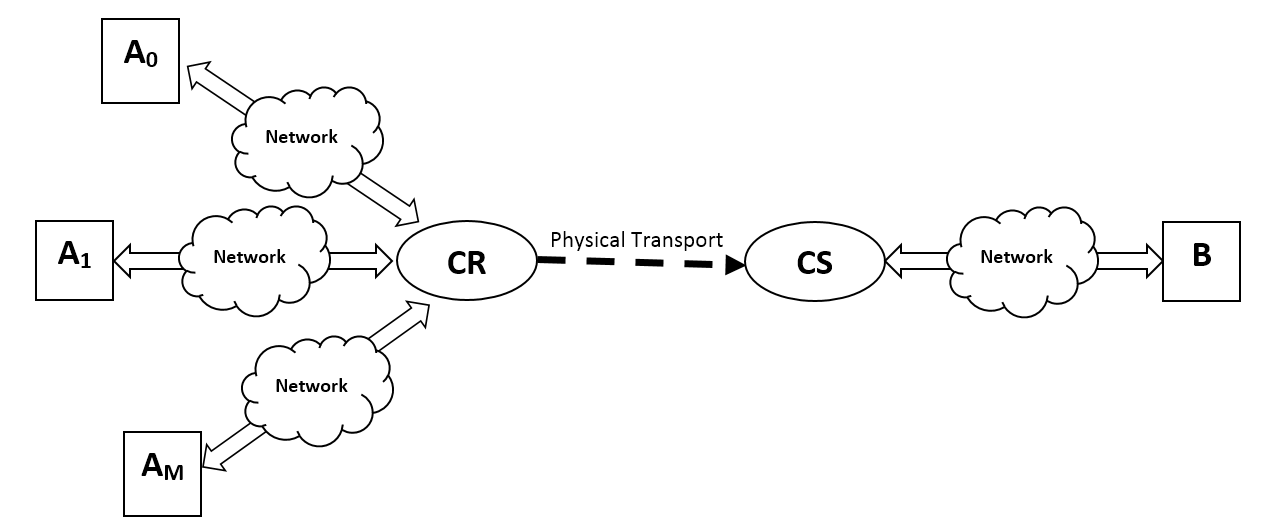
\includegraphics[width=\textwidth,natwidth=1123,natheight=530]{communicationmodel.png}
\caption{Communication Model}
\end{figure}

Above figure illustrates a 3-to-1 communication. The Courier first connects to A$_1$, be the role of $\mathcal{CR}$, and gets A$_1$'s message for B through the connection, then disconnects and transports to A$_2$. It should do the same thing to A$_2$ and then transport to A$_3$. After it collects all data from A$_1$, A$_2$ and A$_3$, it transports to B and be the role of $\mathcal{CS}$ to send all collected messages to B. The networks between Courier and As or B can be any kind of connection and do not to be the same, as long as both entities accept. 

To define different kinds of communication, this protocol consists of 2 sub-protocols - a) Submit protocol: how message is submitted from $\mathcal{A}$ to $\mathcal{C}$; b) Transmit protocol: after $\mathcal{C}$ gets connected with $\mathcal{B}$, how message is transmitted to $\mathcal{B}$. These two sub-protocols ensure the secure transmission of message from $\mathcal{A}$ to $\mathcal{B}$ and they will be analysed in the later part.

\subsubsection*{Behaviour Model}
Generally, all 3 entities in this protocol act as machines who possess their own initial information (described above), take $\mathcal{M}$ as input, and output $\mathcal{M'}$. All honest entities in this protocol should follow the following procedure:
\begin{enumerate}
\item If $\prod \in \mathcal{C}$, initiate the protocol by sending ${\mathcal{M}_0}'$
\item Wait for $\mathcal{M}_1$
\item Receive $\mathcal{M}_1$, decrypt all its ciphertexts and reveal their contents if applicable.
\item Check validity of the contents of $\mathcal{M}_1$ (e.g. check message format, check sender ID, receiver ID, digital signature or MAC, if applicable). If any check violates, immediately report ``Protocol Error" and abort the session.
\item Process the message content (e.g. print the result, stores the contents in local storage).
\item Prepare and send message ${\mathcal{M}_1}'$. If no message to send, abort the session silently.
\item Back to step 2.
\end{enumerate}

However, three entities have different behaviour patterns, they will be specified here, respectively:
\paragraph{Alice $\mathcal{A}$}
\begin{itemize}
\item An entity $a \in \mathcal{A}$ create the message to send, and prepare its meta data. Then it continuously listening to its network, waiting for incoming Couriers.

\item Alice will submit its message to any Courier who request for it. When submitting, the message recipient must be explicitly specified.

\item Alice is allowed to submit any message arbitrary times, to single or multiple Couriers. Alice itself should not care who carries the message, nor how many Couriers carry the message.

\item During an uncompleted session, if no response from Courier for a long time, Alice should be able to detect the timeout, cancel the effects of previous actions in this session and abort the session voluntarily.

\item If the message is not successfully sent, Alice should wait for next Couriers to send this message.
\end{itemize}

\paragraph{Bob $\mathcal{B}$}
\begin{itemize}
\item An entity $b \in \mathcal{B}$ must be continuously listening to its network, waiting for incoming messages.

\item Bob will download all messages from any Courier who transmits. If any message from $\mathcal{A}$ is invalid, Bob simply discards it.

\item Bob will discard all duplicated messages. Duplicated message are defined as messages whose Meta Signature are exactly the same. Because message Meta contains its creator ID and timestamp, same Meta reflects those messages are created by the same entity at the exact same time.

\item During an uncompleted session, if no response from Courier for a long time, Bob should be able to detect the timeout, cancel the effects of previous actions in this session and abort the session voluntarily.
\end{itemize}

\paragraph{Courier $\mathcal{C}$}
\begin{itemize}
\item As Courier's physical transportation is a very complicated task, it is out of the scope of this protocol. It is assumed that Courier is carried by an intelligent agent (such like human) who always knows where the Courier should transport to.

\item Courier should transport to every $a \in \mathcal{A}$ one by one and get their messages if there are.

\item After collect messages from all $a$ in the list, Courier should transport to every $b$ that is the recipient of the Courier and deliver all messages to them. If the receipt from $b$ violates the messages Courier just sent, Courier should resend the messages by restart the session again.

\item Once a full protocol run has been completed, all relative data stored in Courier is expired and should not affect future run of protocol.
\end{itemize}

\subsection*{Adversary Model}
The adversary model in this protocol is mostly derived from Dolev-Yao model which implies ``adversary carries the message" \cite{dolev}. Moreover, the adversary can also do something special in this protocol system. Specifically, adversary $\mathcal{Z}$ has following capabilities:
\begin{itemize}
\item It supervises the whole system, which means it knows when, where and how any two entities are communicating, and it knows which entity possesses what information.
\item It can access/rewrite any message passing through the network.
\item It is a legitimate user of the network and it could be any of 3 entities in this protocol.
\item It can access to all the Courier's data at any stage of the protocol.
\item Any $a \in \mathcal{A}$ or $b \in \mathcal{B}$ will always have the opportunity to be connected by any $c \in \mathcal{C}$.
\end{itemize}

It should be noted that this protocol, same as all other network protocols, is vulnerable to DoS attacks. $\mathcal{Z}$ can always prevent a message from being sent, thus it will not be covered in the security analysis.

\subsection*{Protocol Properties}
\subsubsection*{Submit protocol}
\begin{itemize}
\item $\mathcal{A}$ is authenticated to $\mathcal{CR}$
\item The Integrity of message from $\mathcal{A}$ to $\mathcal{CR}$ is preserved
\item $\mathcal{CR}$ is not able to access the message content
\item $\mathcal{A}$ is able to deny sending any message to $\mathcal{CR}$
\end{itemize}

\subsubsection*{Transmit protocol}
\begin{itemize}
\item $\mathcal{B}$ is authenticated to $\mathcal{CS}$
\item The Integrity of message from $\mathcal{CS}$ to $\mathcal{B}$ is preserved
\item $\mathcal{B}$ is able to deny receiving any message from $\mathcal{CS}$
\end{itemize}

\subsubsection*{On the whole}
\begin{itemize}
\item $\mathcal{A}$ is authenticated to $\mathcal{B}$
\item Confidentiality of message from $\mathcal{A}$ to $\mathcal{B}$ is preserved
\item Integrity of message from $\mathcal{A}$ to $\mathcal{B}$ is preserved
\item $\mathcal{A}$ can not deny sending the message to $\mathcal{B}$
\item $\mathcal{A}$ is able to deny the message content for $\mathcal{B}$
\end{itemize}

\subsection*{Property Proof}
\subsubsection*{Primitives}
Before defining the system model, all the cryptographic primitives used and their corresponding notations in this protocol should be described:
\begin{itemize}
\item Message Authentication Code $\mathcal{MAC}$\\
The MAC function used in this protocol is assumed to be secure in the sense that it has all the properties that a cryptographic hash function possesses and additionally, it resists to existential forgery under chosen-plaintext attack. That is, even if attacker is able to access an oracle which possesses the secret key and generates MACs according to the attacker's input, it is computational infeasible for attacker to guess MACs of other messages (not used to query the oracle).

\item Signature Function $\mathcal{SIGN}$\\
The signature function used in this protocol is assumed to be secure in the sense that it resists existential forgery under an adaptive chosen message attack. \cite{goldwasser}

\item Encryption Function $\mathcal{E}$ and Decryption Function $\mathcal{D}$\\
The notation $\mathcal{E}_k$ denotes an abstraction of all encryption functions, including both symmetric and asymmetric encryptions. Similarly, $\mathcal{D}_k$ represents both symmetric and asymmetric decryption functions. The subscript k denotes the key used for encryption/decryption processes.\\
To assure the security primitives of this protocol, all encryption/decryption schemes used are required to be secure in the sense that without the decryption key, it is computational infeasible for attackers to reveal the plaintext of a cipher with non-negligible probability.

\item Symmetric Key Generator $\mathcal{G}$\\
The symmetric key generator used in this protocol is assumed to be no less secure than a Cryptographically Secure Pseudorandom Number Generator. That is: \\
(a)It should satisfy the next-bit test. That is, given the first k bits of a random sequence, there is no polynomial-time algorithm that can predict the (k+1)th bit with probability of success better than 50\%. \\
(b)It should withstand "state compromise extensions". In the event that part or all of its state has been revealed (or guessed correctly), it should be impossible to reconstruct the stream of random numbers prior to the revelation. Additionally, if there is an entropy input while running, it should be infeasible to use knowledge of the input's state to predict future conditions of the CSPRNG state.\\
Furthermore, the keys generated are required to fit the Symmetric Encryption Scheme described above.
\\
(cite: from wikipedia)
\end{itemize}

\subsubsection*{Submit protocol}
\textbf{THEOREM 1:} $\mathcal{A}$ is authenticated to $\mathcal{CR}$ \\
\emph{$Proof:$} \par
Assuming $\mathcal{G}$ is secure, then $\mathcal{CR}$ is the only entity who knows the randomly generated key $k_C$. Providing $\mathcal{E}_{pk_A}$ scheme is secure, because $k_C$ is encrypted by $pk_A$ before sent out $\mathcal{A}$ will be the only entity who can reveal the encrypted $k_C$. Similarly, providing $\mathcal{MAC}$ scheme is secure, $\mathcal{A}$ is also the only one who can create MESSAGE 2 and its $\mathcal{MAC}_{k_C}$. Thus when (MESSAGE 2, $\mathcal{MAC}_{k_C}$) pair is received by $\mathcal{CR}$ and is verified true, it can be sure this message is created by $\mathcal{A}$. So $\mathcal{A}$ is authenticated to $\mathcal{CR}$.
\\
\\
\textbf{THEOREM 2:} The Integrity of message from $\mathcal{A}$ to $\mathcal{CR}$ is preserved \\
\emph{$Proof:$} \par
Assuming $\mathcal{MAC}$ scheme is secure, any modification of MESSAGE 2 will lead to unpredictable changes in the $\mathcal{MAC}_{k_C}$(MESSAGE 2) and cause its verification to be false. And according to THEOREM 1, no one else but $\mathcal{A}$ can create the message and its valid MAC, message forgery is prevented. As consequence, the message integrity is preserved.
\\
\\
\textbf{LEMMA 1} The message content cannot be revealed by any entity but $\mathcal{B}$ \\
\emph{$Proof:$} \par
Assuming $\mathcal{G}$ is secure, the randomly generated key $k_{AB}$ is only held by $\mathcal{A}$. $k_{AB}$ is encrypted by $\mathcal{E}_{pk_B}$ and sent to $\mathcal{CR}$, so assuming the $\mathcal{E}$ scheme is secure, only $\mathcal{B}$ can decrypt the cipher and reveal $k_{AB}$. As message content is encrypted by $\mathcal{E}_{k_{AB}}$, the only entity can decrypt it is $\mathcal{B}$ because only it knows $k_{AB}$ (other than the message creator). Consequently, only $\mathcal{B}$ can reveal the message content created by $\mathcal{A}$.
\\
\\
\textbf{THEOREM 3:} $\mathcal{CR}$ is not able to access the message content
\\
\emph{$Proof:$} \par
According to LEMMA 1, only $\mathcal{B}$ can reveal the message content, we can easily deduce that $\mathcal{CR}$ is not able to reveal the message content.
\\
\\
\textbf{THEOREM 4:} $\mathcal{A}$ is able to deny sending any message to $\mathcal{CR}$
\\
\emph{$Proof:$} \par
The whole message sent from $\mathcal{A}$ to $\mathcal{CR}$ contains three parts - (1) entity IDs, (2) encrypted message from $\mathcal{A}$ and (3) $\mathcal{MAC}_{k_C}$, if $\mathcal{CR}$ wants to prove the authenticity of the origin of the whole message, it must show that at least one of these three parts can be created only by $\mathcal{A}$. However, all these three parts are forgeable by $\mathcal{CR}$ itself:
\begin{enumerate}
\item entity IDs are plaintexts, thus can be created by $\mathcal{CR}$.
\item as has been proven in LEMMA 1, no entity but $\mathcal{B}$ can reveal the securely generated key $k_{AB}$, so $\mathcal{CR}$ is not able to reveal $\mathcal{SIGN_A}$ or message content, thus the encrypted message is just a block of random data for $\mathcal{CR}$, thus can be created by $\mathcal{CR}$.
\item $\mathcal{MAC}_{k_C}$ can also be created by $\mathcal{CR}$ because $\mathcal{CR}$ has $k_C$ and is able to forge the whole former message.
\end{enumerate}
To sum up, $\mathcal{CR}$ is able to create the whole message itself, it can not convince others the authenticity of the origin of the the message, so $\mathcal{A}$ is able to deny sending the message to $\mathcal{CR}$.

\subsubsection*{Transmit Protocol}
\textbf{THEOREM 5:} $\mathcal{B}$ is authenticated to $\mathcal{CS}$ \\
\emph{$Proof:$} \par
Similar to proof of THEOREM 1, providing $\mathcal{G}$ and $\mathcal{E}$ scheme are secure, only $\mathcal{B}$ knows the symmetric key generated by $\mathcal{CS}$. So, assuming $\mathcal{MAC}$ scheme is secure, if $\mathcal{MAC}_{k_C}$(MESSAGE 1) can be successfully verified by $\mathcal{CS}$, it must be $\mathcal{B}$ who create the MAC. Thus, $\mathcal{B}$ is authenticated to $\mathcal{CS}$.
\\
\\
\textbf{THEOREM 6:} The Integrity of message from $\mathcal{CS}$ to $\mathcal{B}$ is preserved \\
\emph{$Proof:$} \par
Similar to proof of THEOREM 2, any modification on MESSAGE 1 will leads to unpredictable changes in its MAC, and no one else but $\mathcal{B}$ can create the verifiable MAC of arbitrary message. So if $\mathcal{MAC}_{k_C}$(MESSAGE 1) is verified true by $\mathcal{CS}$, it means it is originally created by $\mathcal{B}$ and has not been modified. Thus the message integrity is preserved.
\\
\\
\textbf{THEOREM 7:} $\mathcal{B}$ is able to deny receiving any message from $\mathcal{CS}$ \\
\emph{$Proof:$} \par
Similar to the proof of THEOREM 4, the message from $\mathcal{B}$ is totally forgeable by $\mathcal{CS}$ because it creates the whole MESSAGE 1 and holds $k_C$, it can create $\mathcal{MAC}_{k_C}$(MESSAGE 1) by it own. Therefore $\mathcal{CS}$ cannot prove to others that the MAC is sent from $\mathcal{B}$, $\mathcal{B}$ can deny receiving any message from $\mathcal{CS}$.

\subsubsection*{On The Whole}
\textbf{THEOREM 8:} $\mathcal{A}$ is authenticated to $\mathcal{B}$ \\
\emph{$Proof:$} \par
As $\mathcal{B}$ receives two pieces of data - Meta and Msg, the authentication will be done for both of them separately.\par
\underline{Meta}: Because $\mathcal{B}$ can decrypt the encrypted Meta from $\mathcal{A}$, it can reveal the sender $\mathcal{ID}$ and $k_{AB}$, then it can further decrypt $\mathcal{E}_{k_{AB}}$($\mathcal{SIGN}_A$(Meta)) to get $\mathcal{SIGN}_A$(Meta). Assuming $\mathcal{SIGN}$ scheme is secure, if $\mathcal{B}$ verifies the signature true under $\mathcal{A}$'s public key, $\mathcal{B}$ knows Meta can only be created by $\mathcal{A}$. \par
\underline{Msg}: Assuming $\mathcal{G}$ and $\mathcal{E}$ scheme is secure, only $\mathcal{B}$ can decrypt $\mathcal{E}_{k_{AB}}$($k_{AB}$) and reveal $k_{AB}$ in Meta. Thus only $\mathcal{B}$ (other than $\mathcal{A}$) can create $\mathcal{MAC}_{k_{AB}}$(Msg). So, if (Msg, $\mathcal{MAC}_{k_{AB}}$) pair is verified true by $\mathcal{B}$, $\mathcal{B}$ knows Msg is created by $\mathcal{A}$. \par
To sum up, $\mathcal{A}$ is authenticated to $\mathcal{B}$ as all message sent by $\mathcal{A}$ is authenticated.
\\
\\
\textbf{THEOREM 9:} Confidentiality of the message from $\mathcal{A}$ to $\mathcal{B}$ is preserved\\
\emph{$Proof:$} \par
As proven in THEOREM 3, the message content from $\mathcal{A}$ to $\mathcal{B}$ can not be revealed by any other entities but $\mathcal{B}$, even the Courier itself. So after physical transportation and transmitting message to $\mathcal{B}$, this property still hold. This means only the creator and recipient of the message can reveal its content, so the confidentiality if preserved.
\\
\\
\textbf{THEOREM 10:} Integrity of the message from $\mathcal{A}$ to $\mathcal{B}$ is preserved\\
\emph{$Proof:$} \par
Similar to the proof of THEOREM 6, assuming $\mathcal{G}$ and $\mathcal{E}$ scheme is secure, $\mathcal{B}$ is the only entity who can decrypt $\mathcal{E}_{k_{AB}}$($k_{AB}$) and reveal $k_{AB}$. So when message is received by $\mathcal{B}$, only $\mathcal{A}$ and $\mathcal{B}$ hold $k_{AB}$ and are able to create $\mathcal{MAC}_{k_{AB}}$(Msg). So any forgery will lead to MAC verification fail. Further more, if the Msg is modified, it will lead to unpredictable changes in $\mathcal{MAC}_{k_{AB}}$(Msg) and fail the MAC verification as well. So if (Msg, $\mathcal{MAC}_{k_{AB}}$(Msg)) pair is verified true, the Msg must be created by $\mathcal{A}$, and remain unchanged. Thus the integrity of message from $\mathcal{A}$ to $\mathcal{B}$ is preserved.
\\
\\
\textbf{THEOREM 11:} $\mathcal{A}$ can not deny sending the message to $\mathcal{B}$\\
\emph{$Proof:$} \par
Similar to the proof of THEOREM 8, if $\mathcal{SIGN_A}$ is verified true, it proves the authenticity of the origin of the Meta, so $\mathcal{A}$ can not deny sending the message.
\\
\\
\textbf{THEOREM 12:} $\mathcal{A}$ is able to deny the message content sent to $\mathcal{B}$ \\
\emph{$Proof:$} \par
The message content contains two parts - (1) encrypted message Msg =  $\mathcal{E}_{k_{AB}}$(message) and (2) its MAC $\mathcal{MAC}_{k_{AB}}$(Msg). Because $k_{AB}$ is contained in the Meta and Meta is encrypted under $\mathcal{B}$'s public key, $\mathcal{B}$ is able to reveal $k_{AB}$. Then the whole message content part sent from $\mathcal{A}$ is forgeable by $\mathcal{B}$:
\begin{enumerate}
\item Msg is encrypted under $k_{AB}$, $\mathcal{B}$ can create any Msg it wants.
\item $\mathcal{MAC}_{k_{AB}}$(Msg) also can be created $\mathcal{B}$ because $\mathcal{B}$ can create Msg and hold $k_{AB}$.
\end{enumerate}
As $\mathcal{B}$ can create the whole content part by its own, $\mathcal{B}$ can not prove to others that the message is from $\mathcal{A}$. Thus $\mathcal{A}$ can deny the message content for $\mathcal{B}$.

\begin{thebibliography}{9}
\bibitem{goldwasser}
  Shafi Goldwasser, Silvio Micali, and Ronald Rivest,
  \emph{A digital signature scheme secure against adaptive chosen-message attacks},  SIAM Journal on Computing,
  17(2):281–308,
  Apr. 1988.
  
\bibitem{dolev}
  D. Dolev, A. C. Yao,
  \emph{On the security of public key protocols},
  IEEE trans. on Information Theory,
  IT-29: 198–208,
  1983.
\end{thebibliography}
\end{document}